\subsubsection{Dissecting Outbound Delay} 
\label{mazu-outbound_meas}

We now study the outbound latencies for three different \flowmod\
operations: insertion, modification, and deletion. For each operation, we
examine the latency impact of key factors, including table
occupancy and rule priority.
Before measuring outbound latency, we install a single default low priority
rule which instructs the switch to drop all traffic. We then install a set of
non-overlapping OpenFlow rules that
eth2 interface of our measurement host. For some experiments, we 
systematically vary the rule priorities.


\begin{figure*}[!tb]
	\centering
        \begin{subfigure}[b]{0.24\textwidth}
                \centering
		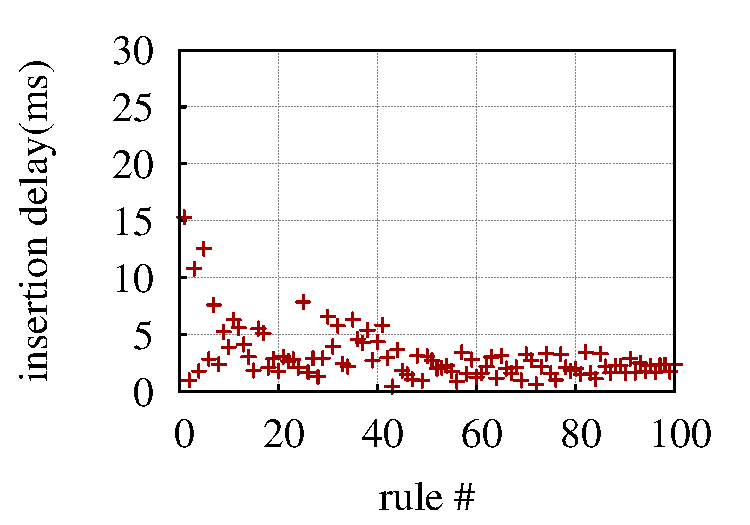
\includegraphics[width=\linewidth]{./figures/mazu/jan27_bcm_add_same_burst_100-eps-converted-to.pdf}
		\caption{burst size 100, same priority}
		\label{fig:bcm_burst_100_same_pri}
	\end{subfigure}
	\centering
        \begin{subfigure}[b]{0.24\textwidth}
                \centering
		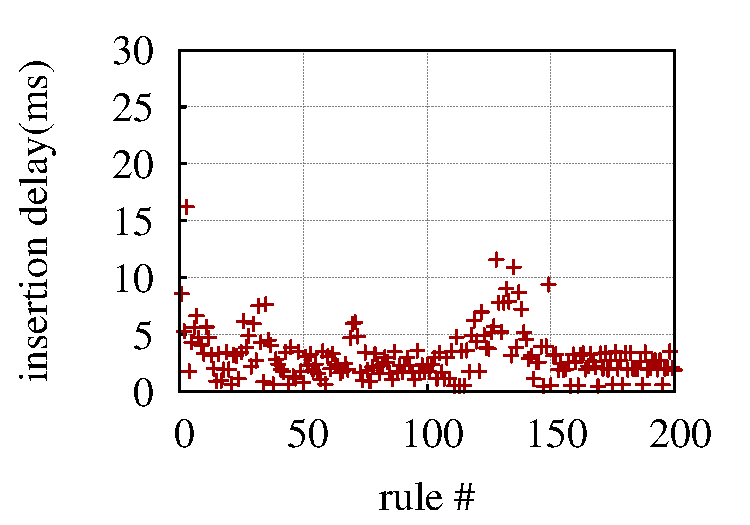
\includegraphics[width=\textwidth]{./figures/mazu/jan27_bcm_add_same_burst_200-eps-converted-to.pdf}
		\caption{burst size 200, same priority}
		\label{fig:bcm_burst_200_same_pri}
	\end{subfigure}
        \centering
        \begin{subfigure}[b]{0.24\textwidth}
                \centering
		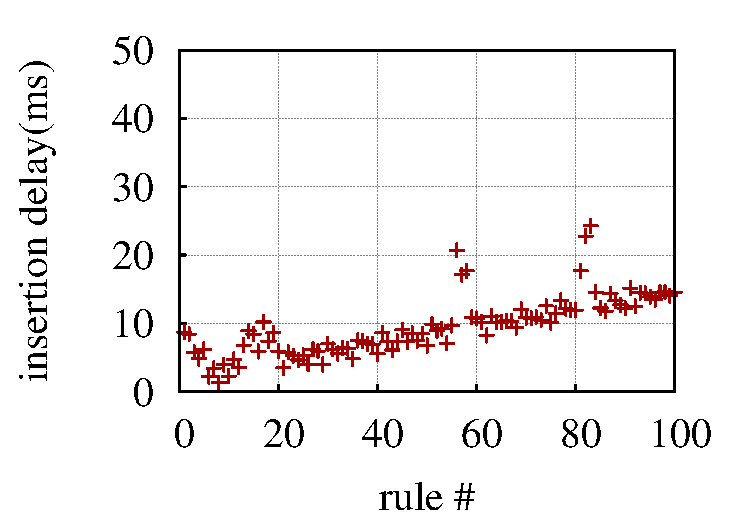
\includegraphics[width=\textwidth]{./figures/mazu/jan27_bcm_add_incr_burst_100-eps-converted-to.pdf}
		\caption{burst size 100, incr. priority}
		\label{fig:bcm_burst_100_incr_pri}
	\end{subfigure}
        \centering
        \begin{subfigure}[b]{0.24\textwidth}
                \centering
		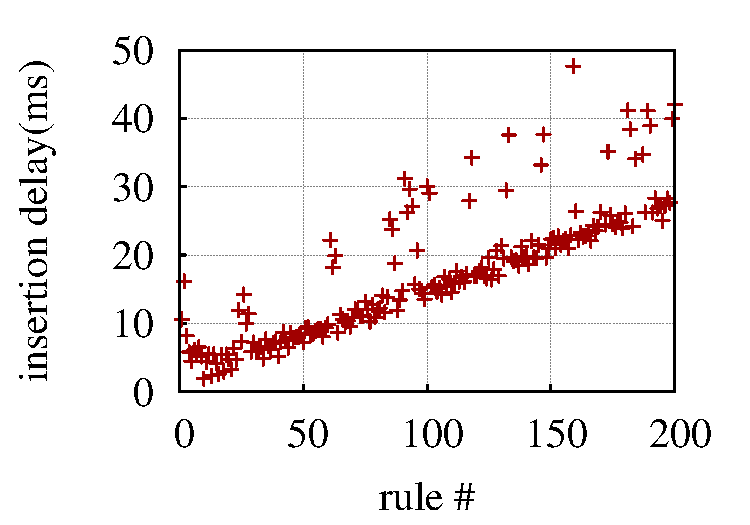
\includegraphics[width=\textwidth]{./figures/mazu/jan27_bcm_add_incr_burst_200-eps-converted-to.pdf}
		\caption{burst size 200, incr. priority}
		\label{fig:bcm_burst_200_incr_pri}
	\end{subfigure}
	\caption{{\bf \BroadcomOne} priority per-rule {\bf insert} latency}
	\label{fig:priority-broadcom-insert}
\end{figure*}


{\emph {We first examine how different rule workloads impact insertion latency}}. We
insert a burst of $B$ rules: $r_1,\cdots,r_B$. Let $T(r_i)$ be the time we
observe the first packet matching $r_i$ emerging from the output port
specified in the rule. We define per-rule insertion latency as $T(r_i)-T(r_{i-1})$.  

\tightparagraph{Rule Complexity} 
To understand the impact of rule complexity (i.e., the number of header 
fields specified in a rule), we install bursts of rules that specify either
2, 8, or 12 fields. In particular, we specify destination IP and EtherType
(others wilcarded) in the 2-field case; input port, EtherType, source and
destination IPs, ToS, protocol, and source and destination ports in the
8-field case; and all supported header fields in the 12-field (exact match)
case. We use a burst size of 100 and all rules have the same priority.
We find that rule complexity {\em does not} impact insertion latency. The
mean per-rule insertion delay for 2-field, 8-field, and exact
match cases is 3.31ms, 3.44ms, and 3.26ms, respectively, for \BroadcomOne.
Similarly, the mean per-rule insertion delay for \Intel, \IBM, and
\BroadcomThree is $\approx$ 1 ms irrespective of the number of fields. 
All experiments that follow use rules with 2 fields.

\tightparagraph{Table occupancy} To understand the impact of table occupancy, we
insert a burst of $B$ rules into a switch that already has $S$ rules
installed. All $B+S$ rules have the same priority. We fix $B$ and
vary $S$, ensuring $B+S$ rules can be accommodated in each switch's hardware
table.
We find that flow table occupancy {\em
does not} impact insertion delay if all rules have the same priority.
Taking $B=400$ as an example, the mean per-rule insertion delay is 3.14ms, 
1.09ms, 1.12ms, and 1.11ms (standard deviation 2.14ms, 1.24ms, 1.53ms, and
        0.18ms) for \BroadcomOne, \BroadcomThree, \IBM
and \Intel, respectively, regardless of the value of $S$. 

\tightparagraph{Rule priority} To understand the effect of rule priority on the
insertion operations, we conducted three different experiments each covering
different patterns of priorities. In each, we insert a burst of $B$ rules
into an empty table ($S=0$); we vary $B$. In the {\em same priority}
experiment, all rules have the same priority. In the {\em increasing} and
{\em decreasing priority} experiments, each rule has a different priority and
the rules are inserted in increasing/decreasing priority order, respectively. 

Representative results for same priority rules are shown in 
\figsref{fig:bcm_burst_100_same_pri}{fig:bcm_burst_200_same_pri} for
$B=100$ and $B=200$, respectively; the switch is \BroadcomOne. For both
burst sizes, the per-rule insertion delay is similar, with medians of 3.12ms
and 3.02ms, and standard deviations of 1.70ms and 2.60ms for $B=100$ and
$B=200$, respectively. The same priority insertion delays on \BroadcomThree,
\IBM, and \Intel are slightly lower, but still similar: mean per-rule
insertion delay is 1.09ms, 1.1ms, and 1.17ms, respectively, for $B=100$.  We
conclude that {\em same priority} rule insertion delay does not vary with burst
size.

In contrast, the per-rule insertion delay of increasing priority rules 
{\em increases linearly} with the number of rules inserted for \BroadcomOne,
\BroadcomThree, and \IBM.
\figsref{fig:bcm_burst_100_incr_pri}{fig:bcm_burst_200_incr_pri} shows this
effect for $B=100$ and $B=200$, respectively, for \BroadcomOne.  Compared with
the same priority experiment, the average per-rule delay is much larger:
9.47ms (17.66ms) vs. 3.12ms (3.02ms), for $B=100$ (200). The results are
similar for \BroadcomThree and \IBM: the average per-rule insertion delay is
7.75ms (16.81ms) and 10.14ms (18.63) for $B=100$ (200), respectively. 
We also observe the slope of the latency increase is constant---for a given
switch---regardless of $B$.

The increasing latency in \BroadcomOne, \BroadcomThree, and \IBM stems from
the TCAM storing high priority rules at low (preferred) memory addresses. Each
rule inserted in the {\em increasing priority} experiments displaces all prior
rules!
Surprisingly, latency does not increase when increasing priority rules are
inserted in \Intel. As shown in \figref{fig:intel_burst_800_incr_pri}, the
median per-rule insertion delay for \Intel is 1.18ms (standard deviation of
1.08ms), even with $B=800$! Results for other values of $B$ are similar.
This shows that the \Intel TCAM architecture is fundamentally different from
\Broadcom and \IBM. Rules are ordered in \Intel's TCAM such that higher
priority rules do not displace existing low priority rules. 
However, displacement does still occur in \Intel. 
\figref{fig:intel_burst_800_decr_pri} shows per-rule insertion latencies for
for {\em decreasing priority} rules for $B=800$. We see two effects: (1) the
latencies alternate between two modes at any given time, and (2) there is a
step-function effect after every 300 or so rules. 
A likely explanation for the former is bus buffering. Since rule insertion is
part of the switch's control path, it is not really optimized for latency.
The latter effect can be explained as follows: Examining the \Intel switch
architecture, we find that it has 24 slices, $A_1\ldots A_{24}$, and each
slice holds 300 flow entries. There exists a consumption order (low-priority
first) across all slices.  Slice $A_i$ stores the $i^{th}$ lowest
priority rule group. If rules are inserted in decreasing priority, $A_1$ is
consumed first until it becomes full. When the next low priority rule is
inserted, this causes one rule to be displaced from $A_1$ to $A_2$.  This
happens for each of the next 300 rules, after which cascaded displacements
happen: $A_1 \rightarrow A_2 \rightarrow A_3$, and so on. We confirmed this
with \Intel.

We observe different trends when inserting {\em decreasing priority} rules
in \BroadcomOne, \BroadcomThree, and \Intel. With \BroadcomOne, we find the
average per-rule insertion delay increases with burst size: 8.19ms for $B=100$
vs. 15.5ms for $B=200$. Furthermore, we observe that the burst of $B$ rules is
divided into several groups, and each group is reordered and inserted in the
TCAM in order of increasing priority. This indicates that \BroadcomOne
firmware reorders the rules and prefers increasing priority insertion.  In
contrast, \BroadcomThree's per-rule insertion delay for decreasing priority
rules is similar to same priority rule insertion: $\approx$ 1ms. Hence, the
\BroadcomThree firmware has been better optimized to handle decreasing
priority rule insertions. The same applies to \Intel: per-rule insertion delay
for decreasing priority rules is similar to same priority rule insertion:
$\approx$ 1.1ms.


\begin{figure*}[!tb]
	\centering
	\begin{subfigure}[b]{0.40\textwidth}
                \centering
		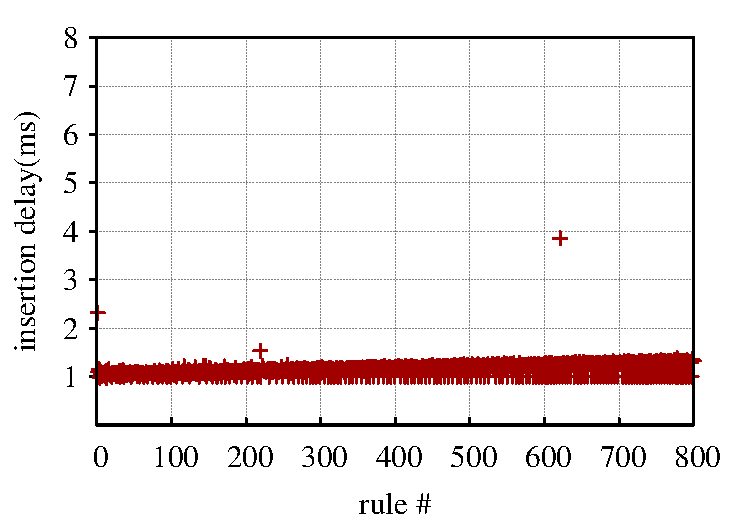
\includegraphics[width=\textwidth]{./figures/mazu/jan27_intel_incr_burst_800-eps-converted-to.pdf}
		\caption{burst size 800, incr. priority}
		\label{fig:intel_burst_800_incr_pri}
	\end{subfigure}
        \begin{subfigure}[b]{0.40\textwidth}
                \centering
		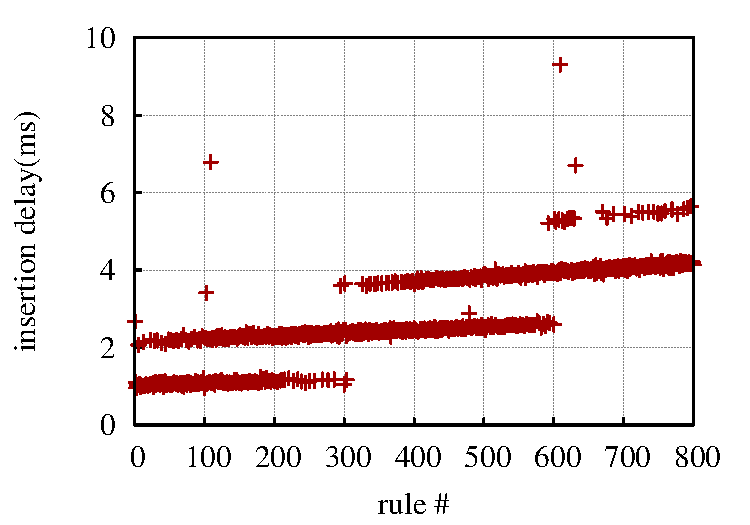
\includegraphics[width=\textwidth]{figures/mazu/jan27_intel_empty_800L_decr_delta-eps-converted-to.pdf}
		\caption{burst size 800, decr. priority}
		\label{fig:intel_burst_800_decr_pri}
	\end{subfigure}
	\caption{{\bf Intel} priority per-rule {\bf insert}} 
	\label{fig:priority-intel-insert}
\end{figure*}


\tightparagraph{Priority and table occupancy combined effects} 
We now study the combined impact of rule priority and table occupancy.
We conduct two experiments: For the first experiment, the table starts with
$S$ high priority rules, and we insert $B$ low priority rules.  For the
second experiment, the priorities are inverted.
For both experiments, we measure the total time to install all rules in the
burst, $T(r_B)-T(r_1)$.

\begin{figure*}[!t]
	\centering
        \begin{subfigure}[b]{0.40\textwidth}
                \centering
		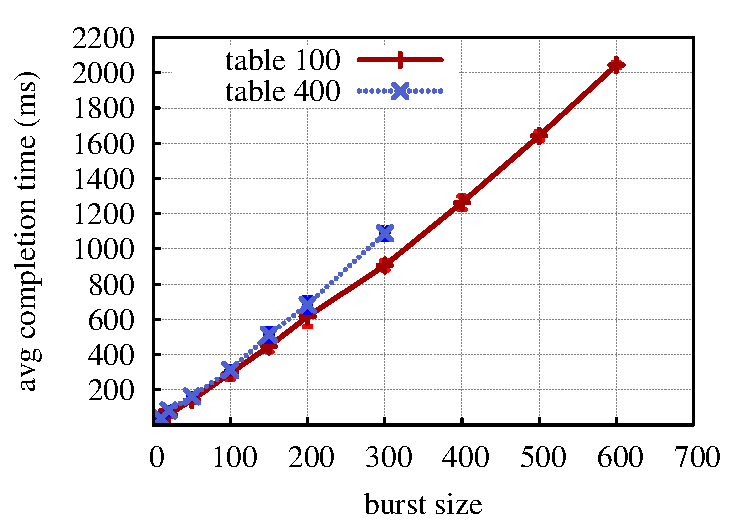
\includegraphics[width=\textwidth]{./figures/mazu/bcm_two_pri_high_low_burstB-eps-converted-to.pdf}
		\caption{insert low priority rules into a table with high priority rules}
		\label{fig:bcm_outbound_two_pri_high_low_burstB}
	\end{subfigure}
        \begin{subfigure}[b]{0.40\textwidth}
                \centering
		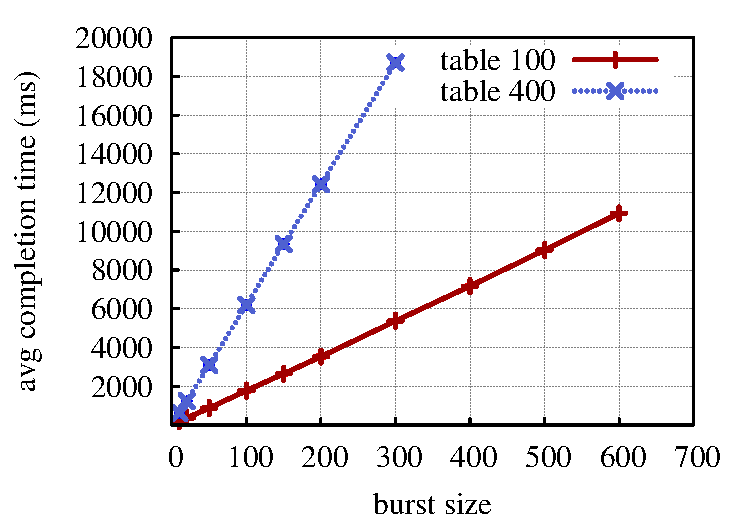
\includegraphics[width=\textwidth]{./figures/mazu/bcm_two_pri_low_high_burstB-eps-converted-to.pdf}
		\caption{insert high priority rules into a table with low priority rules}
		\label{fig:bcm_outbound_two_pri_low_high_burstB}
	\end{subfigure}
	\caption{Overall completion time on {\bf \BroadcomOne}.  Initial table occupancy is S high (low) priority rules; insert a burst of low (high) priority rules. Averaged over 5 runs. }
	\label{fig:burst-completion-time}
\end{figure*}


For \BroadcomOne, \BroadcomThree, and \IBM, we expect that as long as the same
number of rules are displaced, the completion time for different values of
$S$ should be the same.
Indeed, from \figref{fig:bcm_outbound_two_pri_high_low_burstB} (for
\BroadcomOne), we see that even with 400 high priority rules in the
table, the insertion delay for the first experiment is no different from the
setting with only 100 high priority rules in the table. In contrast, in
\figref{fig:bcm_outbound_two_pri_low_high_burstB}, newly inserted high
priority rules will displace low priority rules in the table, so when
$S=400$ the completion time is about 3x higher than $S=100$.
%\fixme{added IBM below}
For \IBM (not shown), inserting 300 high priority rules into a table with 400
low priority rules takes more than 20 seconds.  


%For \Intel, we also run the same two experiments as for Broadcom. 
For \Intel, the results are similar to same priority rule insertion. This
indicates that \Intel uses different TCAM organization schemes than the
\Broadcom and \IBM switches.  %\fixme{changed}
%optimizes for rule priority better than \BroadcomOne. 
 
\tightparagraph{Summary and root causes}
We observe that: (1) rule complexity does not affect insertion delay; (2)
same priority insertions in \BroadcomOne, \BroadcomThree, \Intel and \IBM are fast
and not affected by flow table occupancy; and (3) priority insertion patterns
can affect insertion delay very differently. For \Intel, increasing priority
insertion is similar to same priority insertion, but decreasing priority 
incurs much higher delay. For \BroadcomThree and \IBM the behavior is inverted:  
decreasing priority insertion is similar to same priority insertion and increasing priority insertion incurs higher delay. For \BroadcomOne, 
insertions with different priority patterns are all much higher than
insertions with same priority. 
Key root causes for observed latencies are: (1) how rules are organized in the TCAM, and (2) the number of slices. {\em Both of these are intrinsically tied to switch hardware.} Even in the best case (\Intel), per-rule insertion latency of 1ms is higher than what native TCAM hardware can support (100M updates/s~\cite{estan:private}). Thus, in addition to the above two causes, there appears to be an {\em intrinsic switch software overhead} contributing to all latencies.



{\emph {We now study modification operations}}. As before, we use bursts of rules and
a similar definition of latency.

\tightparagraph{\bf Table occupancy} To study the impact of table
occupancy, we pre-insert $S$ rules into a switch,
all with the same priority. We then modify one rule at a time by changing the
rule's output port, sending modification requests back to back. 

\begin{figure*}[!tb]
	\centering
        \begin{subfigure}[b]{0.40\textwidth}
                \centering
		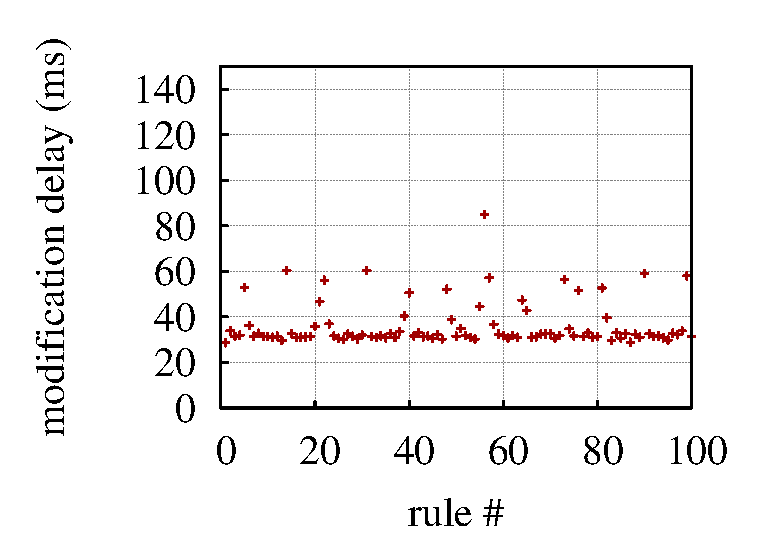
\includegraphics[width=\textwidth]{./figures/mazu/jan27_bcm_mod_same_burst_100_imc.eps}
		\caption{100 rules in table}
		\label{fig:bcm_mod_same_burst_100}
	\end{subfigure}
        \begin{subfigure}[b]{0.40\textwidth}
                \centering
		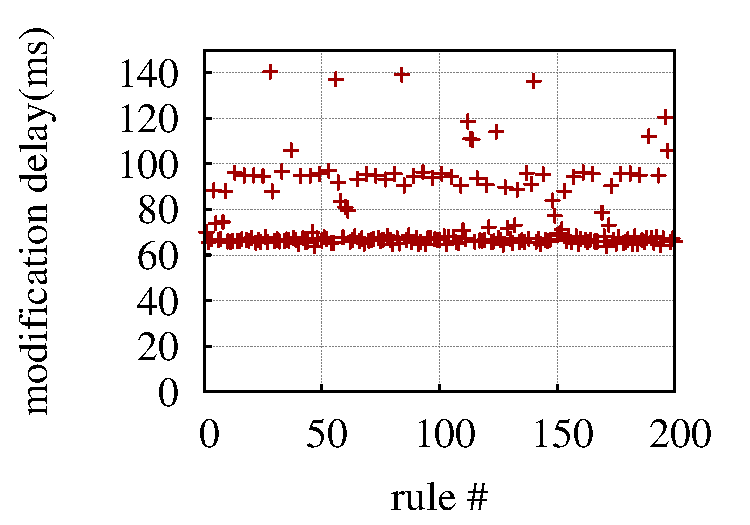
\includegraphics[width=\textwidth]{./figures/mazu/jan27_bcm_mod_same_burst_200-eps-converted-to.pdf}
		\caption{200 rules in table}
		\label{fig:bcm_mod_same_burst_200}
	\end{subfigure}
	\caption{{\bf \BroadcomOne} per-rule {\bf mod.} latency, same priority}
	\label{fig:occupancy-broadcom-modify}
\end{figure*}
 
Per-rule modification delay for \BroadcomOne when $S=100$ and $S=200$ are shown in
\figsref{fig:bcm_mod_same_burst_100}{fig:bcm_mod_same_burst_200}, respectively. We
see that the per-rule delay
is more than 30 ms for $S=100$. When we double the number of rules,
$S=200$, latency doubles as well. It grows
linearly with $S$ (not shown). Note that
this latency is much higher than the corresponding
insertion latency (3.12ms per rule).
\IBM's per-rule modification latency is also affected significantly by the table occupancy---
the per-rule modification latencies for $S=100$ and $S=200$ are 18.77ms and 37.13ms, respectively.
In contrast, \Intel and \BroadcomThree  have lower modification delay,
and it does not vary with table occupancy. For \Intel (\BroadcomThree) the
per-rule modification delay for both $S=100$ and $S=200$ is around 1 ms (2ms)
for all modified rules, similar to (2X more than) same priority insertion delay. 


\tightparagraph{Rule Priority} We conduct two experiments on each switch to
study the impact of rule priority. In
each experiment, we insert $B$ rules into an empty table ($S = 0$). In the 
{\em increasing} priority experiments, the rules in the table each have a
unique priority, and we send back-to-back modification requests for
rules in increasing priority order. We do the opposite in the {\em
decreasing priority} experiment. We vary $B$.%  across

\begin{figure*}[!t]
	\centering
	\begin{subfigure}[b]{0.40\textwidth}
                \centering
		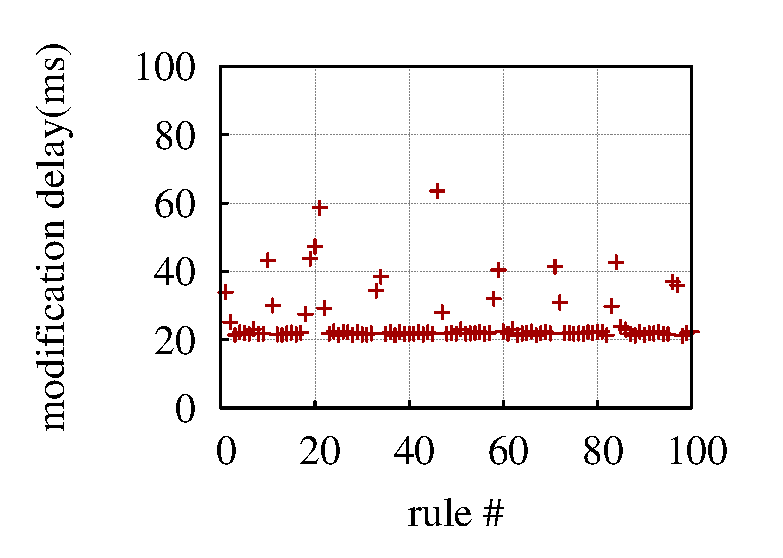
\includegraphics[width=\textwidth]{./figures/mazu/jan27_bcm_mod_incr_burst_100.eps}
		\caption{burst size 100, incr. priority}
		\label{fig:bcm_mod_incr_burst_100}
	\end{subfigure}
        \begin{subfigure}[b]{0.40\textwidth}
                \centering
		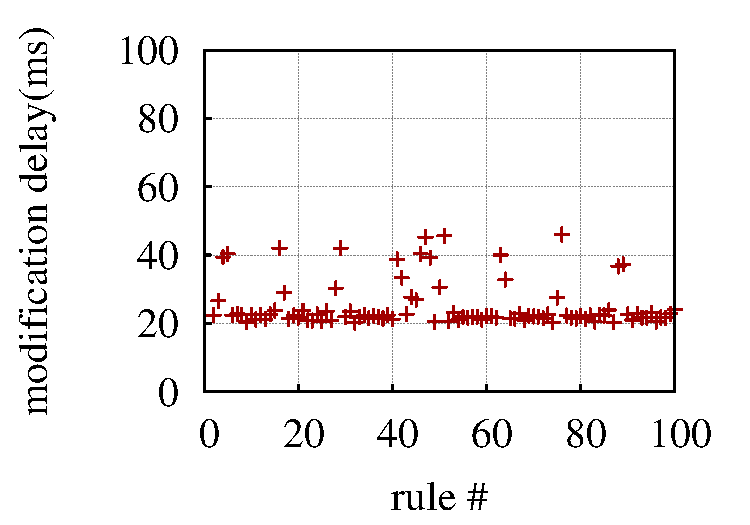
\includegraphics[width=\textwidth]{./figures/mazu/jan27_bcm_mod_decr_burst_100-eps-converted-to.pdf}
		\caption{burst size 100, decr. priority}
		\label{fig:bcm_mod_decr_burst_100}
	\end{subfigure}
	\caption{{\bf \BroadcomOne} priority per-rule {\bf modification} latency}
	\label{fig:priority-broadcom-modify}
\end{figure*}

\figsref{fig:bcm_mod_incr_burst_100}{fig:bcm_mod_decr_burst_100} show the results for the increasing and decreasing priority experiments, respectively, for
$B=100$ on \BroadcomOne. In both cases, we see: (1) the per-rule modification delay is similar
across the rules, with a median of 25.10ms and a standard deviation of
6.74ms, and (2) the latencies are identical across the experiments. 
We similarly observe that priority does not affect modification delay in
\BroadcomThree, \Intel and \IBM (not shown).


\tightparagraph{Summary and root causes}
We conclude that the per-rule modification latency on \BroadcomOne and \IBM is 
impacted purely by table occupancy, not by rule priority structure.
For \BroadcomThree and \Intel, the per-rule modification delay 
is independent of rule priority, table occupancy, and burst size;
\BroadcomThree's per-rule modification delay is 2X higher than insertion.
Conversations with Broadcom indicated that TCAM modification should ideally be fast and independent of table size, 
so the underlying cause appears to be less optimized switch software in \BroadcomOne. Indeed, our measurements with \BroadcomThree show that this issue has (at least partly) been fixed.


{\emph {Finally, we now study the latency of rule deletions}}.
We again use bursts of operations.
$T(r_i)$ denotes the time we stop observing packets matching rule $r_i$
from the intended port of the rule action. We define deletion latency
as $T(r_i)-T(r_{i-1})$.

\begin{figure*}[!t]
	\centering
        \begin{subfigure}[b]{0.40\textwidth}
                \centering
		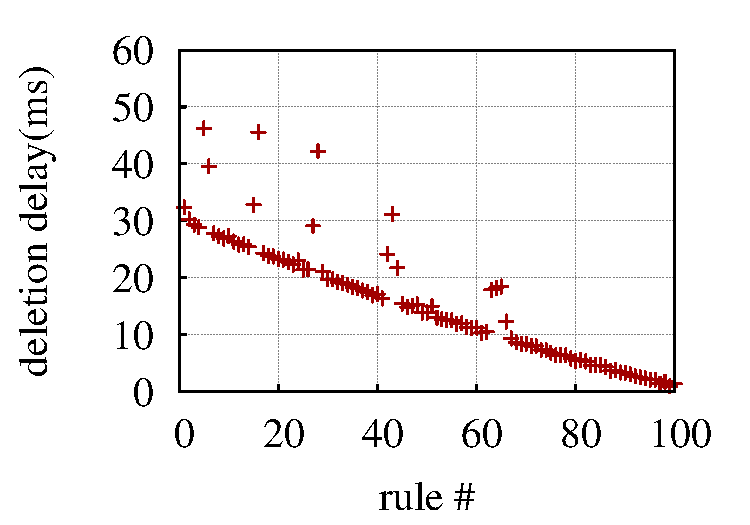
\includegraphics[width=\textwidth]{./figures/mazu/jan27_bcm_del_same_burst_100-eps-converted-to.pdf}
		\caption{100 rules in table}
		\label{fig:bcm_del_same_burst_100}
	\end{subfigure}
        \begin{subfigure}[b]{0.40\textwidth}
                \centering
		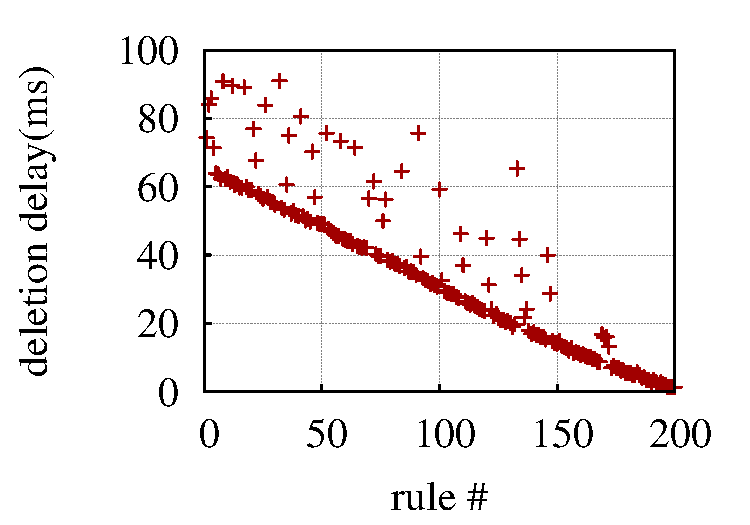
\includegraphics[width=\textwidth] {./figures/mazu/jan27_bcm_del_same_burst_200-eps-converted-to.pdf}
		\caption{200 rules in table}
		\label{fig:bcm_del_same_burst_200}
	\end{subfigure}
	\caption{ {\bf \BroadcomOne} per-rule {\bf del.} latency, same priority}
	\label{fig:occupancy-broadcom-deletion}
\end{figure*}

\begin{figure*}[!t]
	\centering
        \begin{subfigure}[b]{0.40\textwidth}
                \centering
		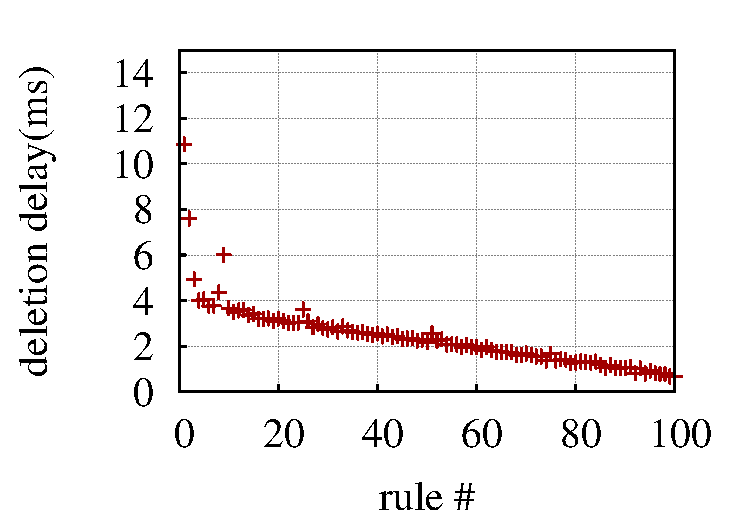
\includegraphics[width=\textwidth]{./figures/mazu/jan27_intel_del_same_burst_100-eps-converted-to.pdf}
		\caption{100 rules in table}
		\label{fig:intel_del_same_burst_100}
	\end{subfigure}
        \begin{subfigure}[b]{0.40\textwidth}
                \centering
		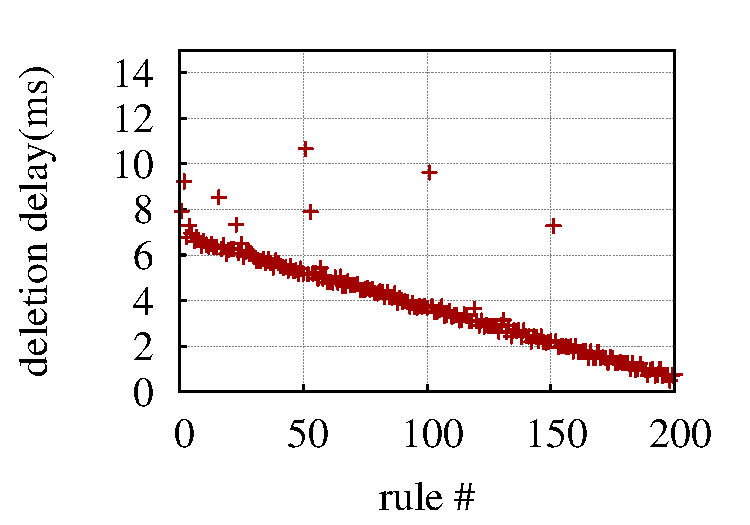
\includegraphics[width=\textwidth]{./figures/mazu/jan27_intel_same_burst_200-eps-converted-to.pdf}
		\caption{200 rules in table}
		\label{fig:intel_del_same_burst_200}
	\end{subfigure}
	\caption{{\bf \Intel} per-rule {\bf del.} latency, same priority}
	\label{fig:occupancy-intel-deletion}
\end{figure*}

\tightparagraph{Table Occupancy} We pre-insert $S$ rules into a switch, all with
the same priority. We then delete one rule at a time, sending deletion
requests back-to-back. The results for \BroadcomOne at $S=100$ and $S=200$
are shown in \figsref{fig:bcm_del_same_burst_100}{fig:bcm_del_same_burst_200},
respectively. We see that per rule deletion delay decreases as the table occupancy drops. We see a similar trend for Intel (\figsref{fig:intel_del_same_burst_100}{fig:intel_del_same_burst_200}) \BroadcomThree and \IBM (not shown).


\begin{figure*}[!t]
	\centering
        \begin{subfigure}[b]{0.40\textwidth}
                \centering
		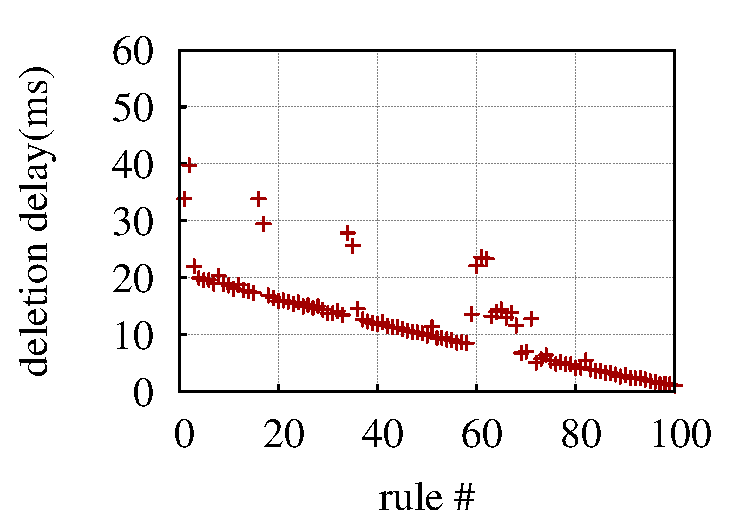
\includegraphics[width=\textwidth]{./figures/mazu/jan27_bcm_del_incr_burst_100-eps-converted-to.pdf}
		\caption{increasing priority}
		\label{fig:bcm_del_incr_burst_100}
	\end{subfigure}
        \begin{subfigure}[b]{0.40\textwidth}
                \centering
		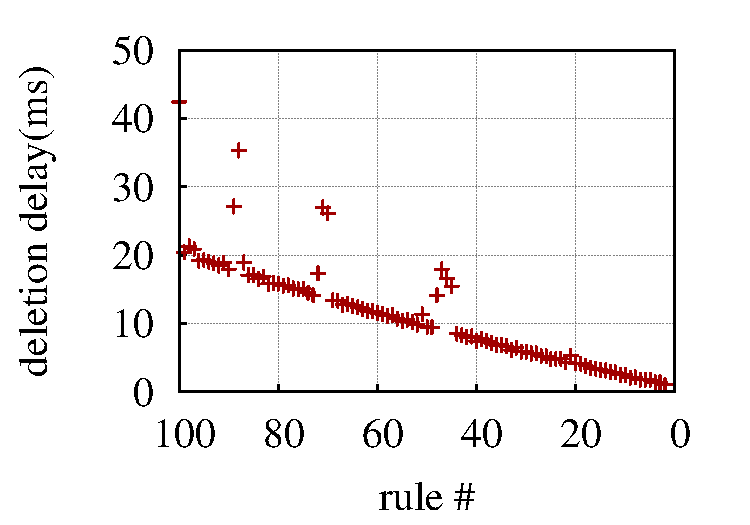
\includegraphics[width=\textwidth]{./figures/mazu/jan27_bcm_del_decr_burst_100-eps-converted-to.pdf}
		\caption{decreasing priority}
		\label{fig:bcm_del_decr_burst_100}
	\end{subfigure}
	\caption{{\bf \BroadcomOne} priority per-rule {\bf del.} latency, 
    B=100}
	\label{fig:priority-broadcom-deletion}
\end{figure*}

\begin{figure*}[!t]
	\centering
        \begin{subfigure}[b]{0.40\textwidth}
                \centering
		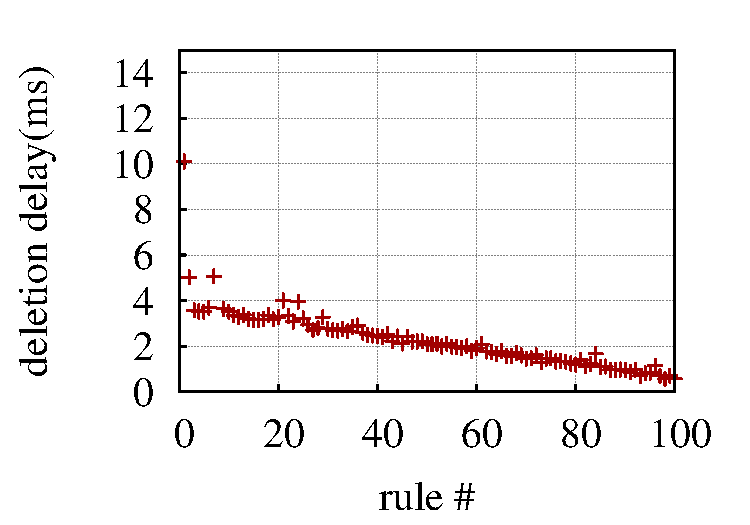
\includegraphics[width=\textwidth]{./figures/mazu/jan27_intel_del_incr_burst_100-eps-converted-to.pdf}
		\caption{increasing priority}
		\label{fig:intel_del_incr_burst_100}
	\end{subfigure}
        \begin{subfigure}[b]{0.40\textwidth}
                \centering
		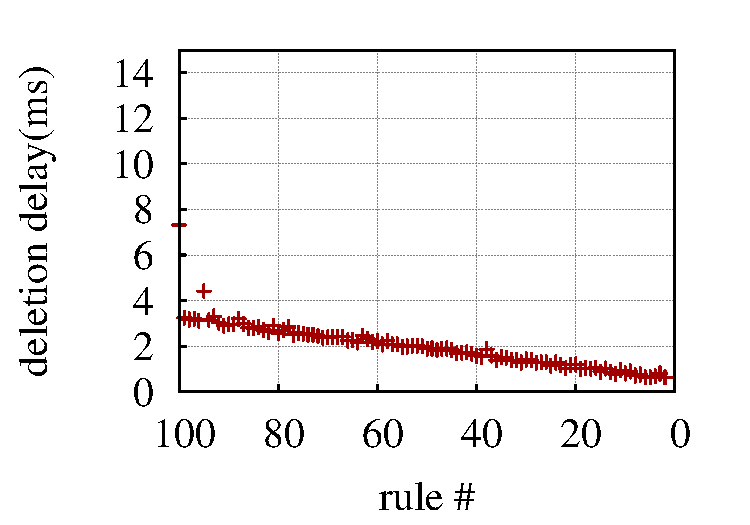
\includegraphics[width=\textwidth]{./figures/mazu/jan27_intel_del_decr_burst_100-eps-converted-to.pdf}
		\caption{decreasing priority}
		\label{fig:intel_del_decr_burst_100}
	\end{subfigure}
	\caption{{\bf Intel} priority per-rule {\bf del.} latency, B=100}
	\label{fig:priority-intel-deletion}
\end{figure*}


\tightparagraph{Rule Priorities} We start with $B$ existing rules in the switch, 
and delete one rule at a time
in increasing and decreasing priority order. 
For all switches (\BroadcomOne and \Intel shown in
\figsref{fig:priority-broadcom-deletion}{fig:priority-intel-deletion},
respectively)
deletion is not affected by the priorities of rules in the table or the order 
of deletion.

\tightparagraph{\bf Root cause} Since deletion delay decreases with rule number 
in all cases, we conclude that deletion is incurring TCAM reordering.
We also observe that processing rule timeouts at the switch does not
noticeably impact \flowmod operations. Given these two observations, we
recommend allowing rules to time out rather than explicitly deleting them, if
possible.


